\begin{frame}{Content Overview}
  \footnotesize
    \begin{enumerate}
        \item<2-> Motivation, Background, and Objectives
        \visible<3->{
        \begin{itemize}
            {\footnotesize
            \item The Impossible Trinity of Modeling (ITM)
            \item The Impossible Trinity of Optimal Control (ITOC)}
        \end{itemize}}
        \item<4-> Addressing the ITM
        \item<5-> Unified Control-Theoretic Training
        \item<6-> Addressing the ITOC
        \item<7-> Conclusions and Future Work
    \end{enumerate}
\end{frame}

\section{Motivation, Background, and Objectives}

\begin{frame}{Content Overview}
  \footnotesize
    \begin{enumerate}
        \item \colorbox{yellow!70}{\textbf{Motivation, Background, and Objectives}}
        \item \textcolor{gray!50}{Addressing the Impossible Trinity of Modeling (ITM)}
        \item \textcolor{gray!50}{Unified Control-Theoretic Training}
        \item \textcolor{gray!50}{Addressing the Impossible Trinity of Optimal Control (ITOC)}
        \item \textcolor{gray!50}{Conclusions and Future Work}
    \end{enumerate}
\end{frame}

% \begin{frame}{\large Motivation: Simulation and Control of Hypersonic Systems}
%     \footnotesize
%     \begin{columns}
%         \begin{column}{0.6\textwidth}
%             \centering
%             \only<1>{
%                 \begin{figure}
%                     \centering
%                     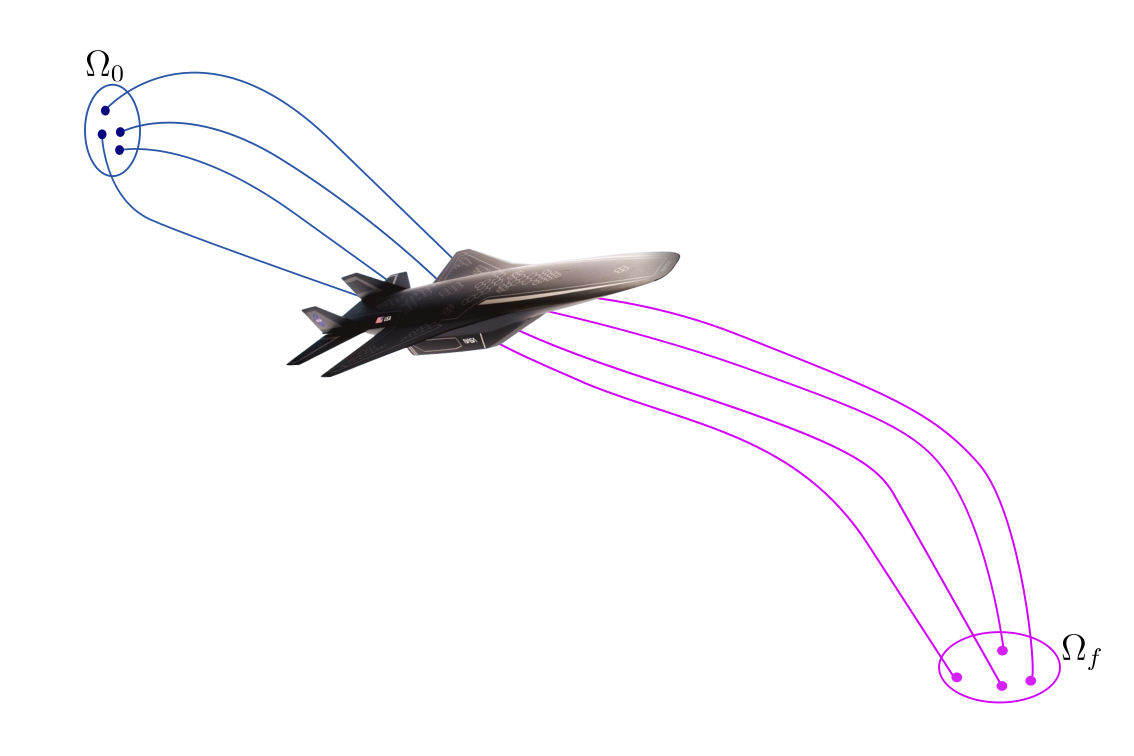
\includegraphics[width=0.9\textwidth]{../figs/introduction/motivating_example_1.png}
%                 \end{figure}}
%             \only<2>{
%                 \begin{figure}
%                     \centering
%                     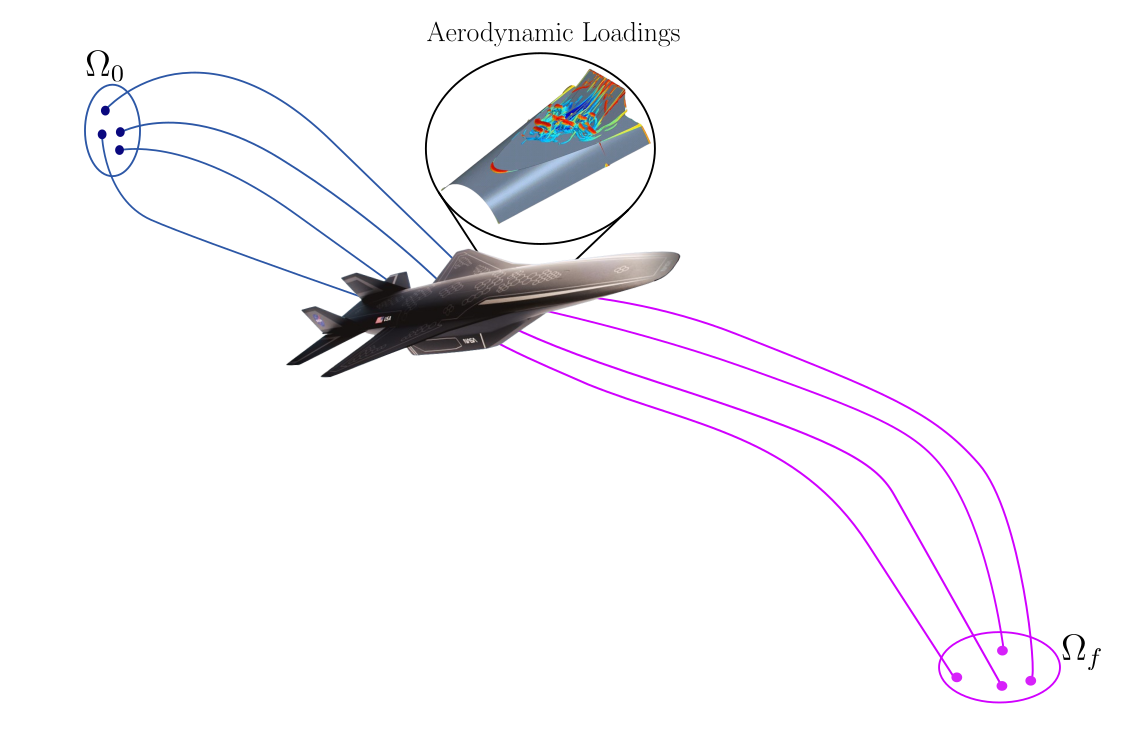
\includegraphics[width=0.9\textwidth]{../figs/introduction/motivating_example_2.png}
%                 \end{figure}}
%             \only<3>{
%                 \begin{figure}
%                     \centering
%                     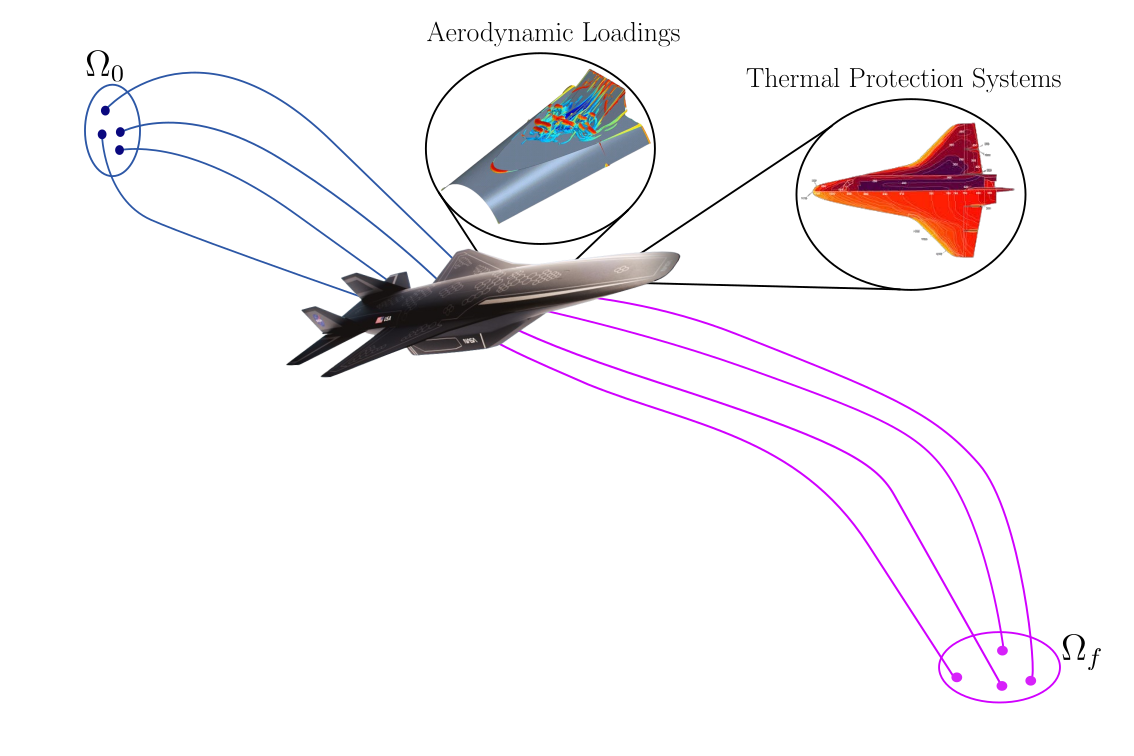
\includegraphics[width=0.9\textwidth]{../figs/introduction/motivating_example_3.png}
%                 \end{figure}}
%             \only<4>{
%                 \begin{figure}
%                     \centering
%                     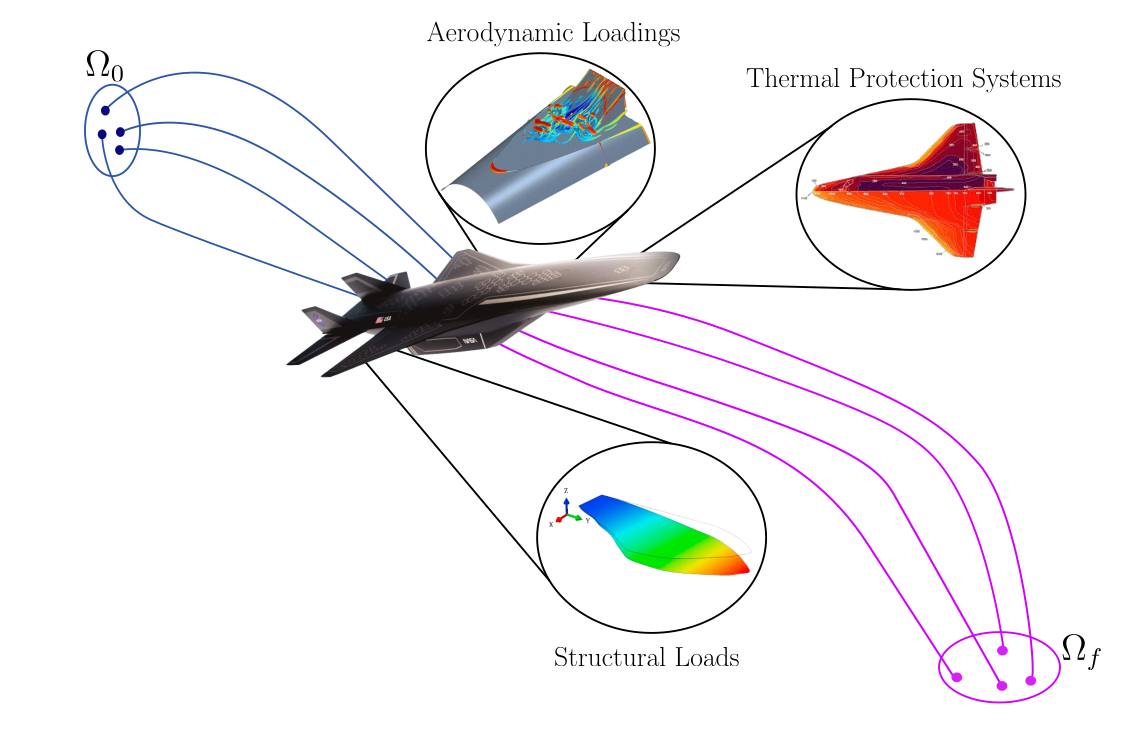
\includegraphics[width=0.9\textwidth]{../figs/introduction/motivating_example_4.png}
%                 \end{figure}}
%             \only<5->{
%                 \begin{figure}
%                     \centering
%                     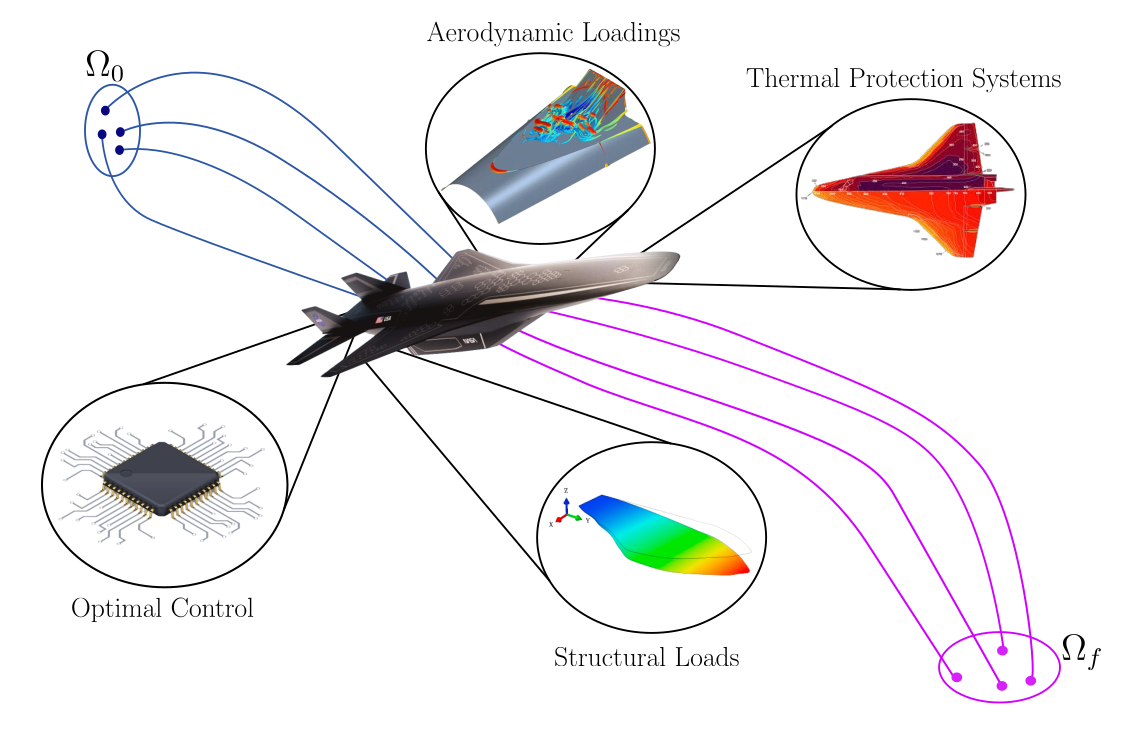
\includegraphics[width=0.9\textwidth]{../figs/introduction/motivating_example_5.png}
%                 \end{figure}}
%         \end{column}
%         \hspace*{-0.4in}
%         \begin{column}{0.45\textwidth}
%             \centering
%             \visible<6->{
%             \begin{graybox}{Simulation}
%                 \visible<7->{
%                 e.g., aero-thermo-servo-elasticity,}
%                 \vspace*{-0.1in}
%                 \begin{align*}
%                     \visible<8->{
%                     \dot{\vu} &= \mathbf{F}\left(\vu;\mathbf{p}\right)}\\
%                     \visible<9->{
%                     \vz_{\text{HF}} &= \mathbf{H}\left(\vu;\vp\right)}\\
%                     \visible<10->{
%                     \vu(t_0) &= \vu_0(\vp)}
%                 \end{align*}
%             \end{graybox}}
%             \visible<11->{
%             \begin{graybox}{Optimal Control/Design}
%                 \visible<12->{
%                 e.g., optimal control problem,}
%                 \vspace*{-0.1in}
%                 \begin{align*}
%                     \visible<13->{
%                     \min_{\vp} \: \mathcal{J} = \int_{t_0}^{t_f} & \ell\left(\vu,\mathbf{p}\right) dt}\\
%                     \visible<14->{
%                     \text{s.t.} \: \quad \dot{\vu} &= \mathbf{F}\left(\vu;\mathbf{p}\right)}\\
%                     \visible<15->{
%                     \mathbf{Q} &\geq \mathbf{g}\left(\vu(t),t;\mathbf{p}\right)}
%                 \end{align*}
%             \end{graybox}}
%         \end{column}
%     \end{columns}
%     \visible<6->{
%     \begin{center}
%         {\tiny
%         $\vu$: high-dimensional states, $\vF$: non-linear dynamics $\vp$: design/control parameters, $\vz_{\text{HF}}$: high-fidelity outputs, $\mathcal{J}$: cost functional, $l$: running cost, $\mathbf{Q}$: safety bound, $\vg$: constraint function}
%     \end{center}}
% \end{frame}

\begin{frame}{\large Motivation: Simulate and Optimally Control Hypersonic Systems}
    \footnotesize
    \only<2>{
        \begin{figure}
            \centering
            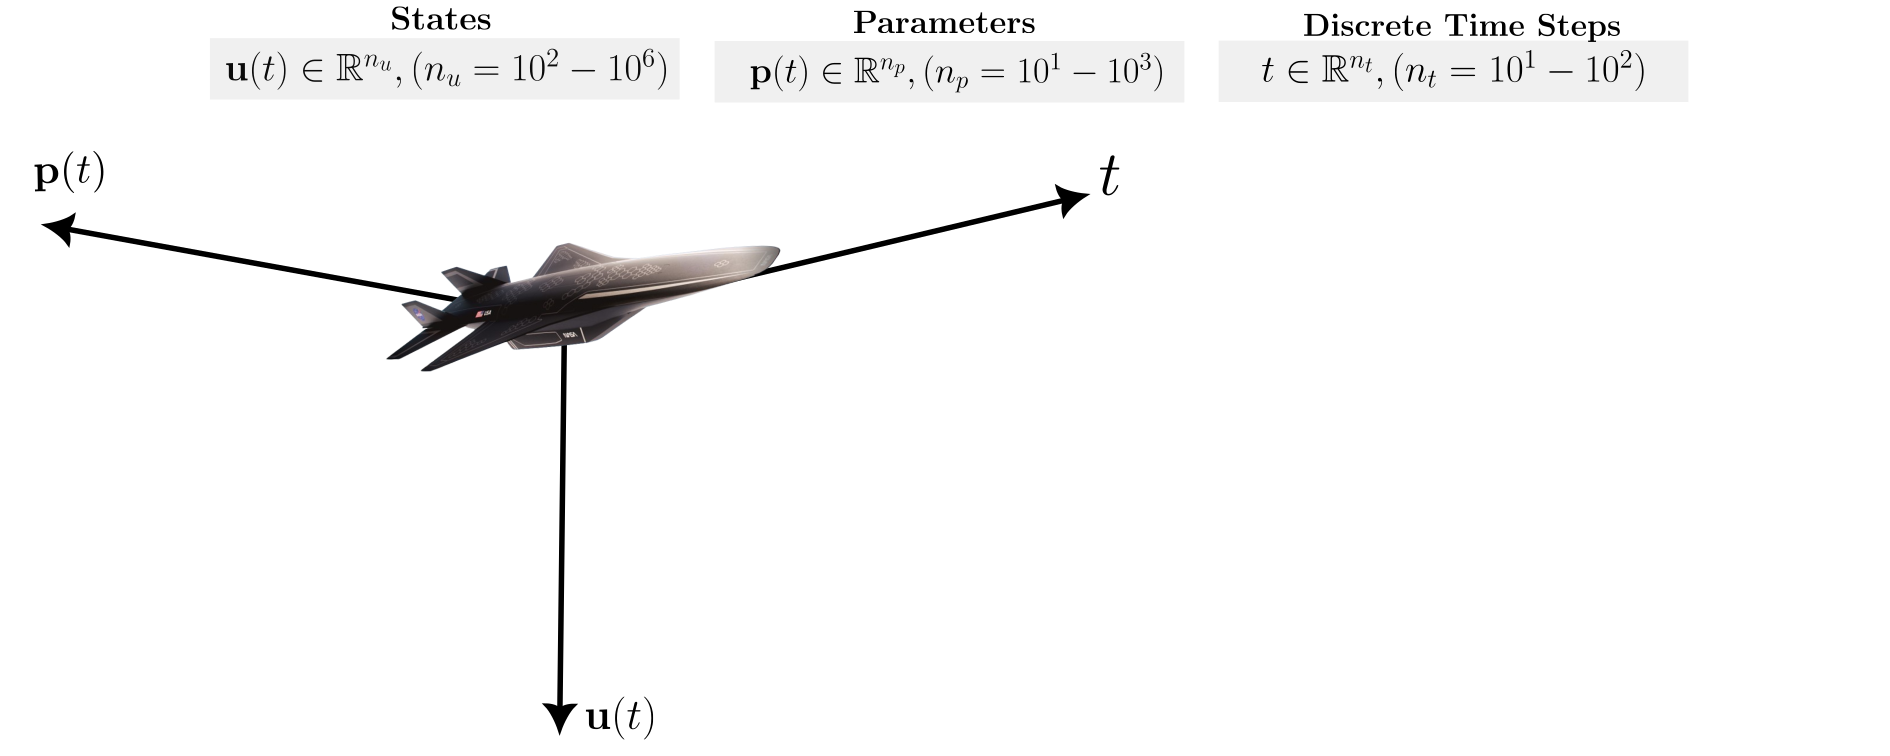
\includegraphics[width=0.95\textwidth]{../figs/introduction/problem_space_1.png}
        \end{figure}}
    \only<3>{
        \begin{figure}
            \centering
            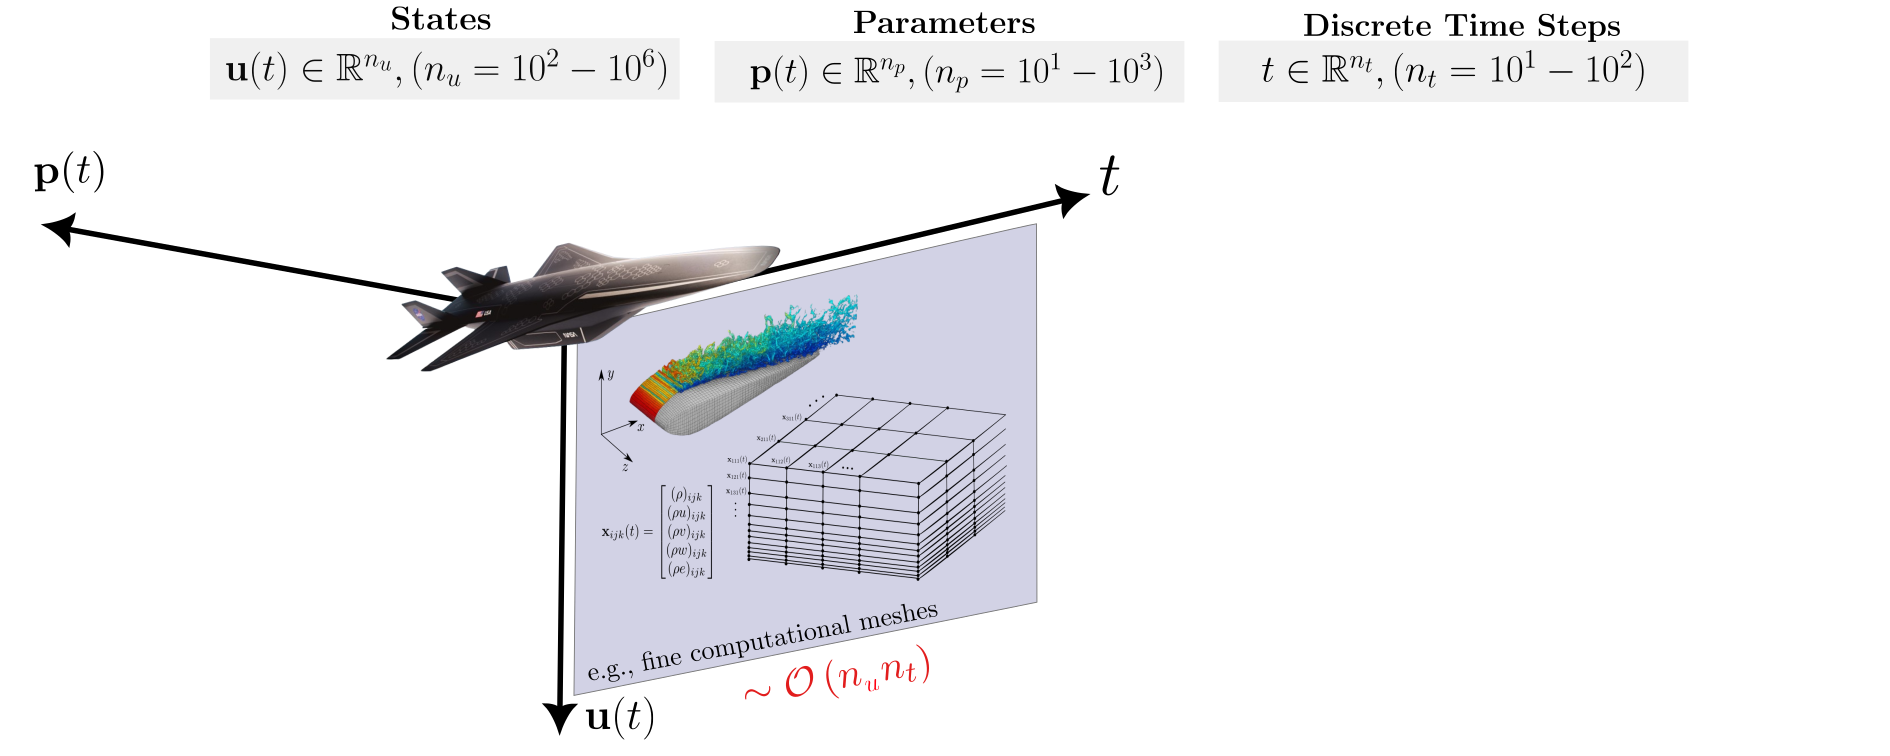
\includegraphics[width=0.95\textwidth]{../figs/introduction/problem_space_2.png}
        \end{figure}}
    \only<4>{
        \begin{figure}
            \centering
            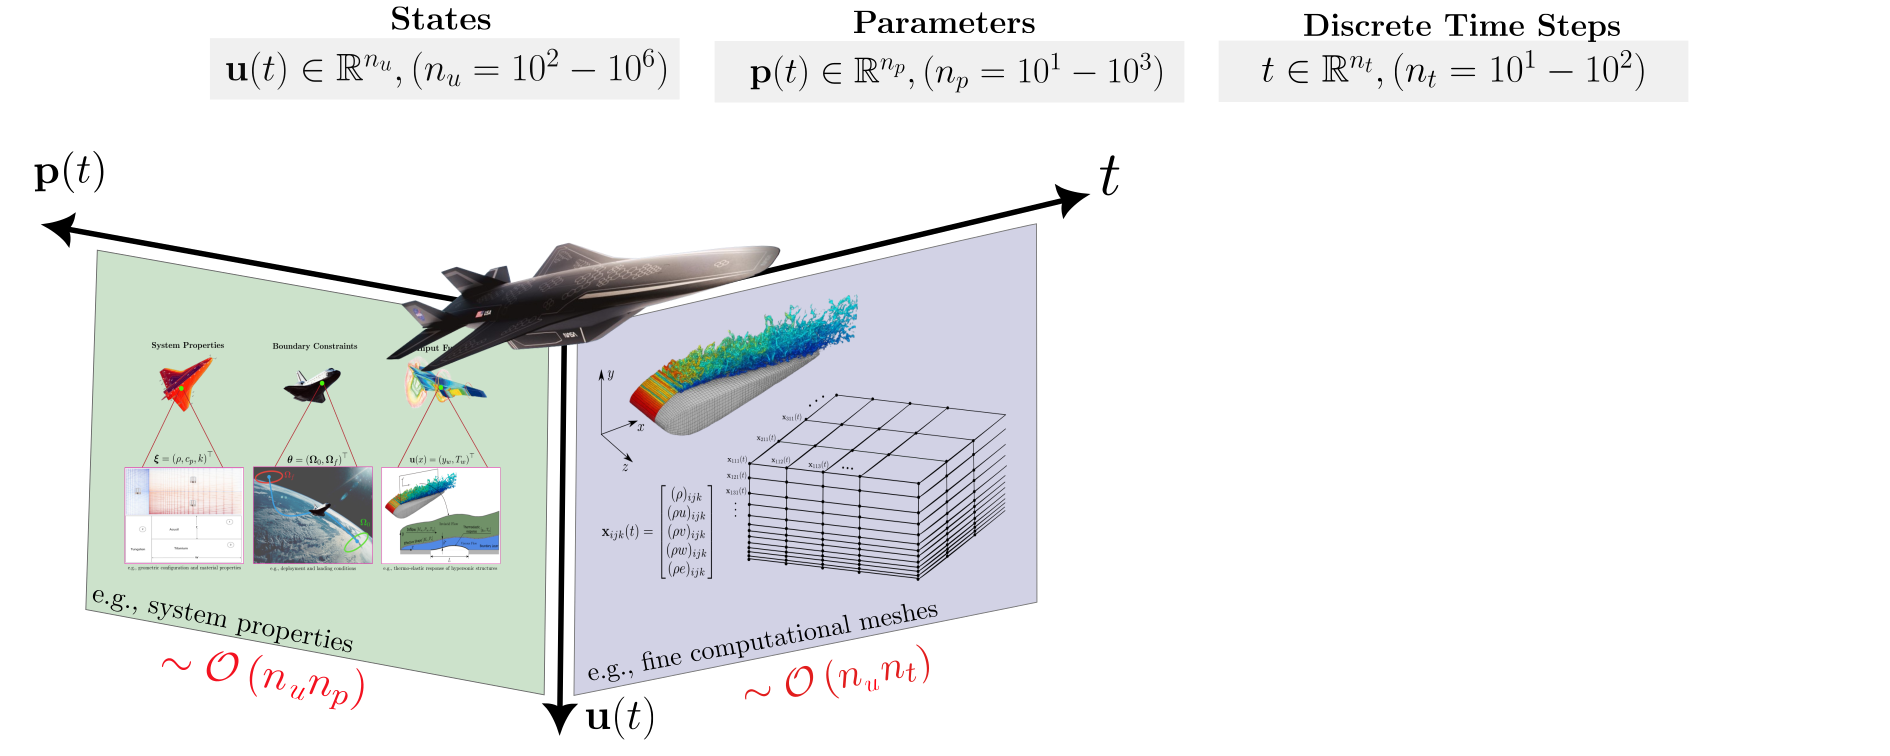
\includegraphics[width=0.95\textwidth]{../figs/introduction/problem_space_3.png}
        \end{figure}}
    \only<5>{
        \begin{figure}
            \centering
            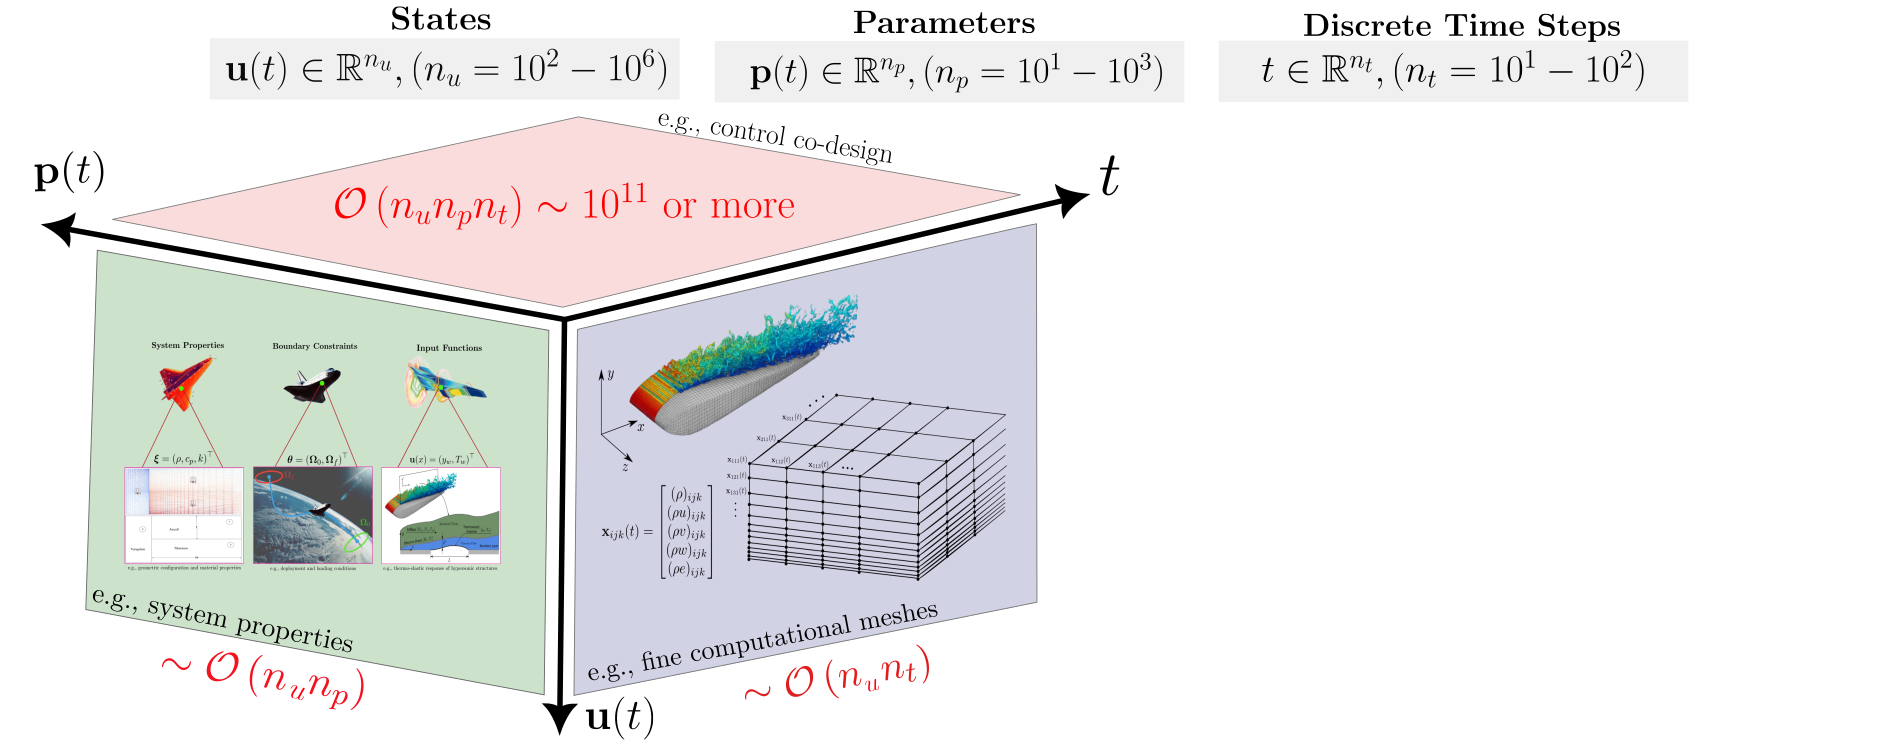
\includegraphics[width=0.95\textwidth]{../figs/introduction/problem_space_4.png}
        \end{figure}}
    \only<6>{
        \begin{figure}
            \centering
            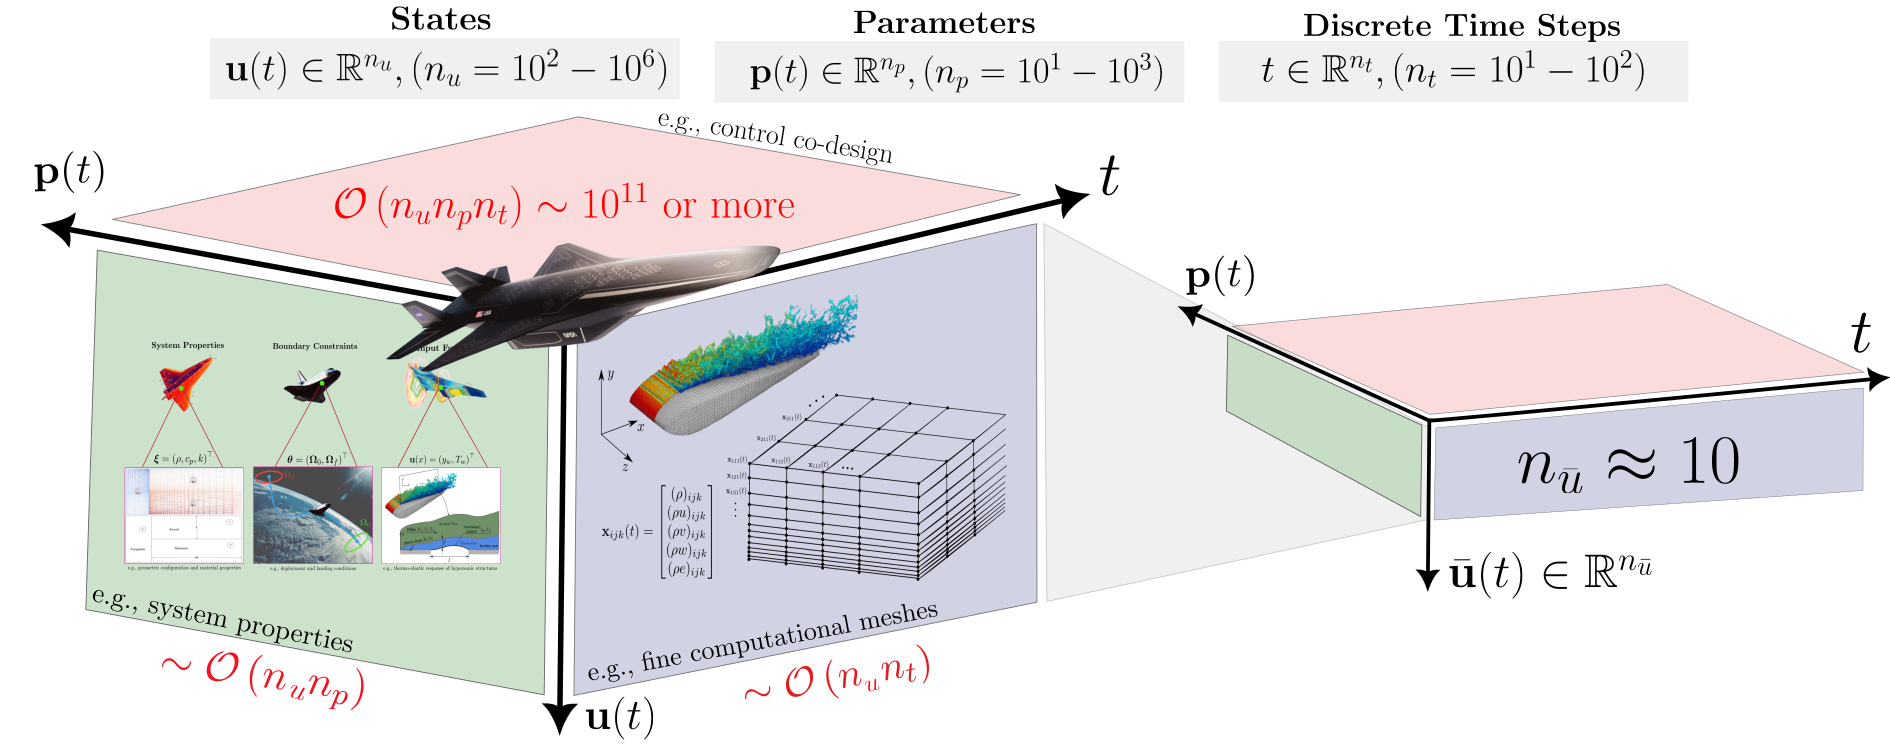
\includegraphics[width=0.95\textwidth]{../figs/introduction/problem_space_5.png}
        \end{figure}}
    \only<7>{
        \begin{figure}
            \centering
            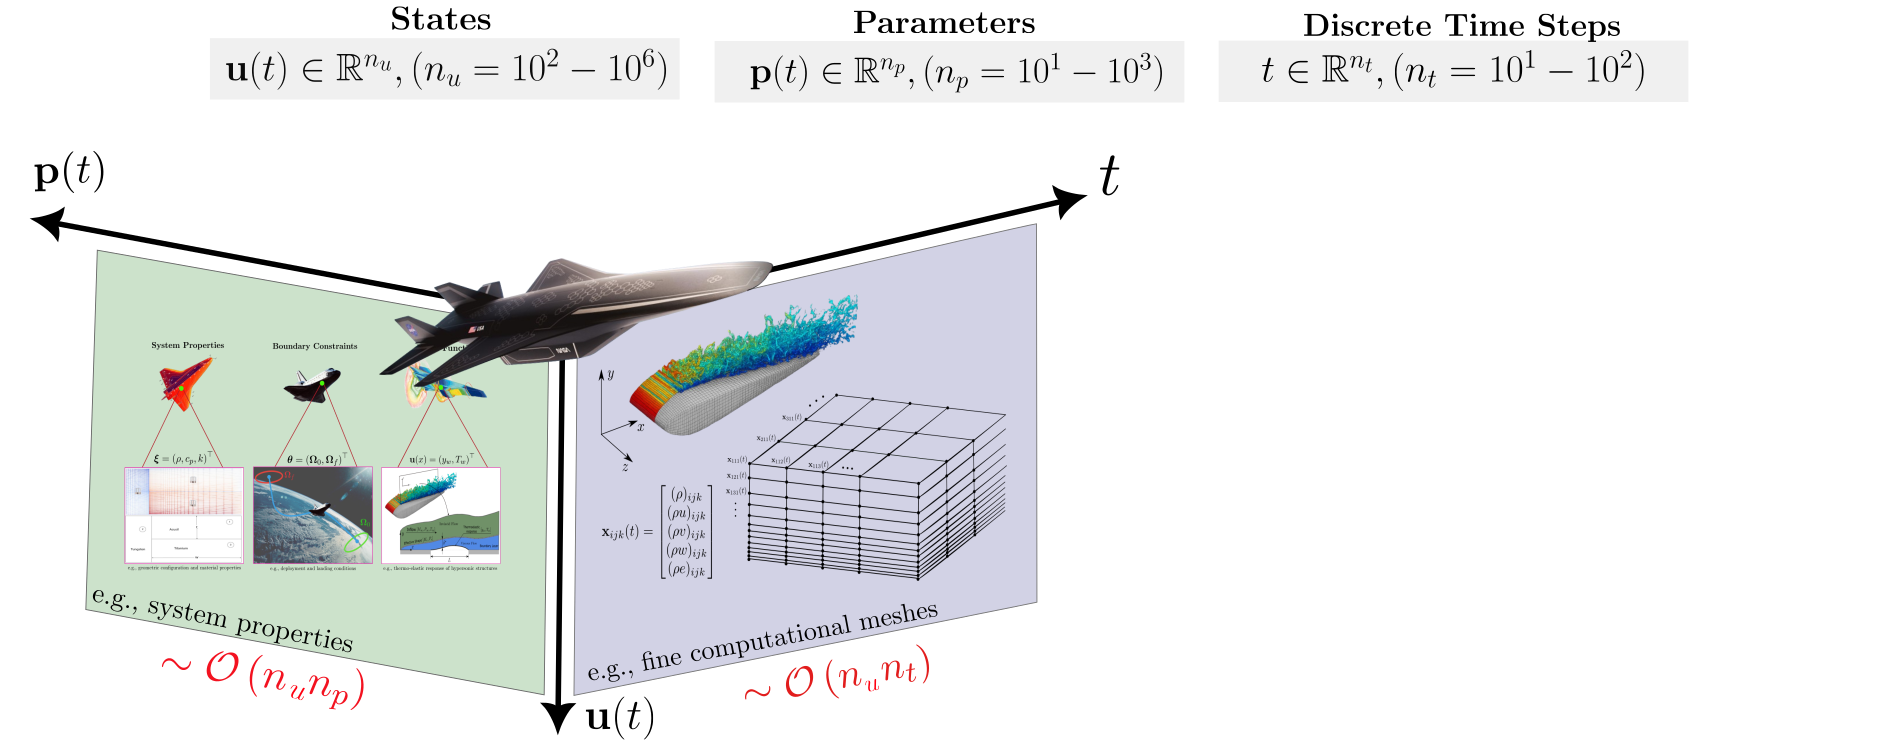
\includegraphics[width=0.95\textwidth]{../figs/introduction/problem_space_6.png}
        \end{figure}}
    \only<8->{
        \begin{figure}
            \centering
            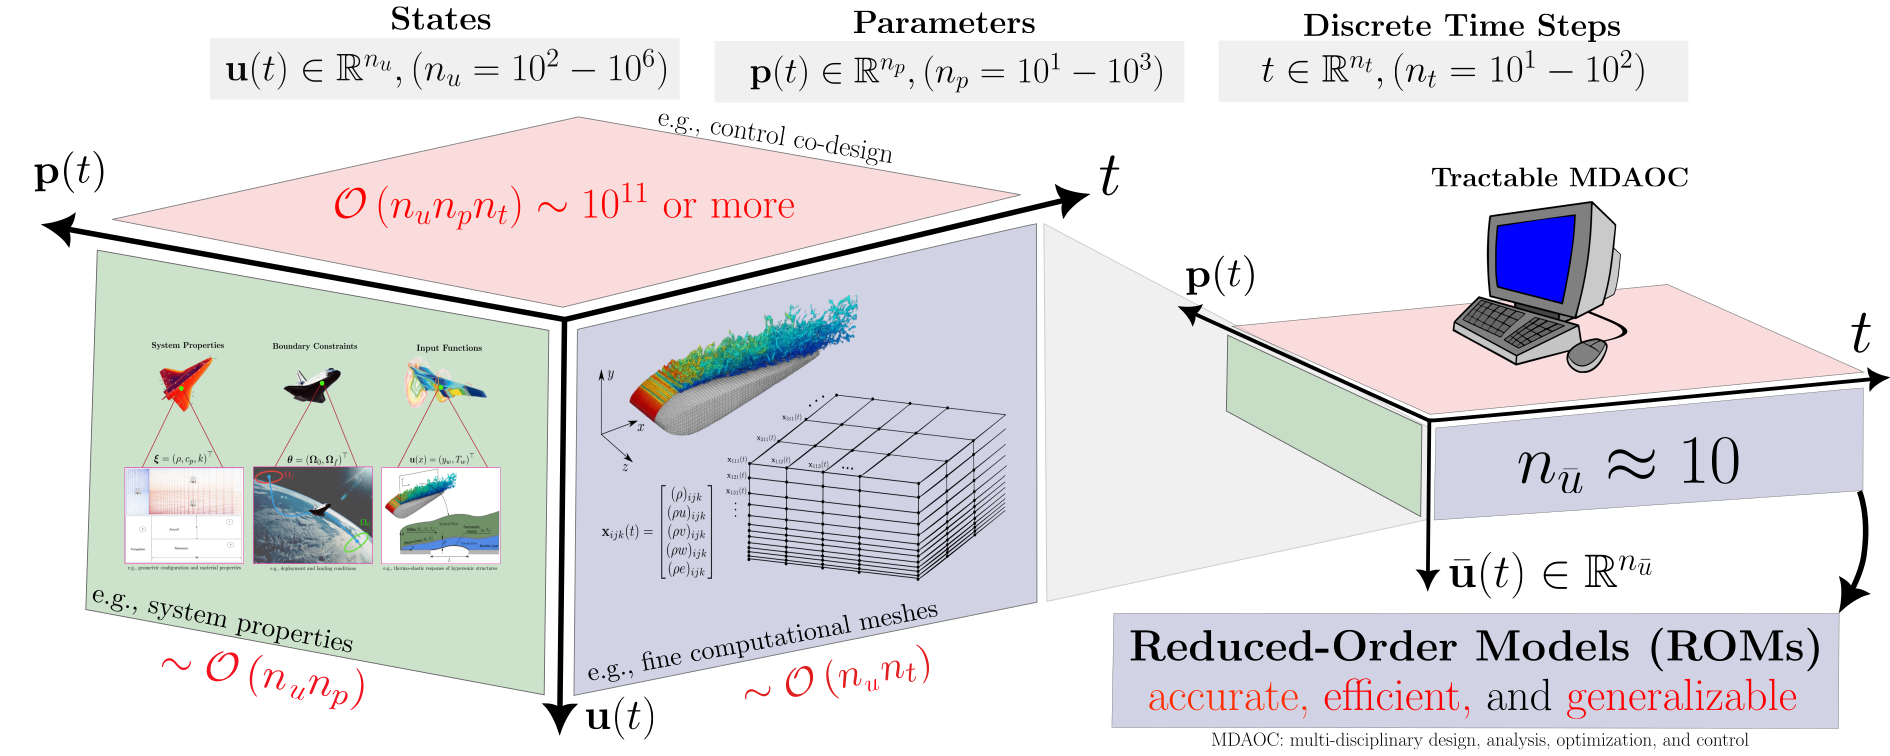
\includegraphics[width=0.95\textwidth]{../figs/introduction/problem_space_7.png}
        \end{figure}}
\end{frame}

\begin{frame}{\large ITM in Simulation: Balancing Accuracy, Efficiency, and Generalizability with Little Data}
    \footnotesize
    \hspace*{-0.1in}
    \begin{columns}
        \begin{column}{0.65\textwidth}
            \only<1-2>{
                \begin{figure}
                    \centering
                    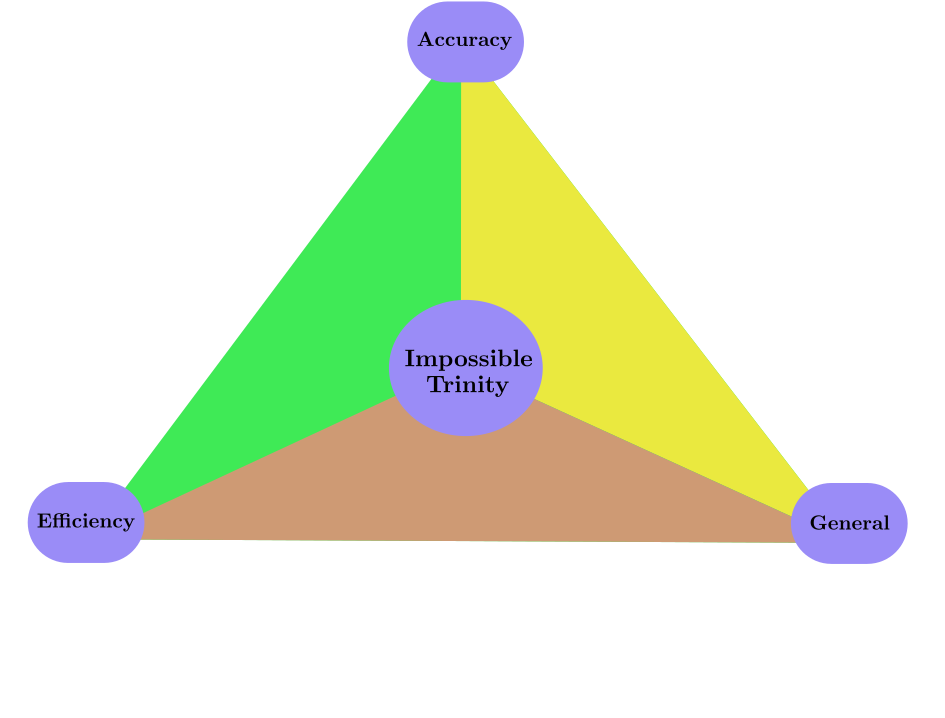
\includegraphics[width=0.8\textwidth]{../figs/introduction/itm_1.png}
                \end{figure}}
            \only<3>{
                \begin{figure}
                    \centering
                    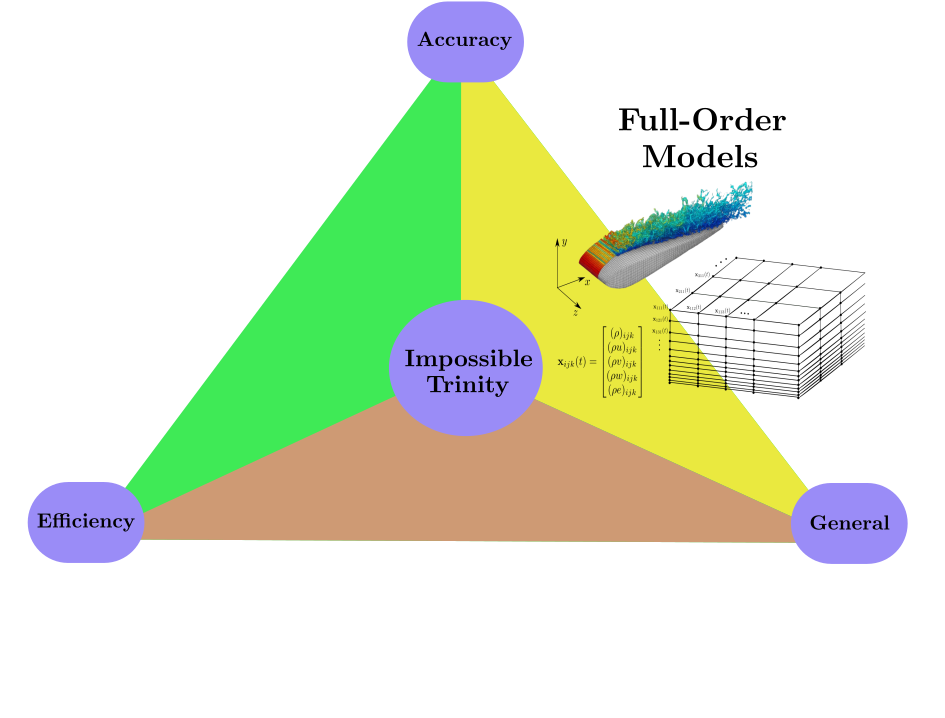
\includegraphics[width=0.8\textwidth]{../figs/introduction/itm_2.png}
                \end{figure}}
            \only<4>{
                \begin{figure}
                    \centering
                    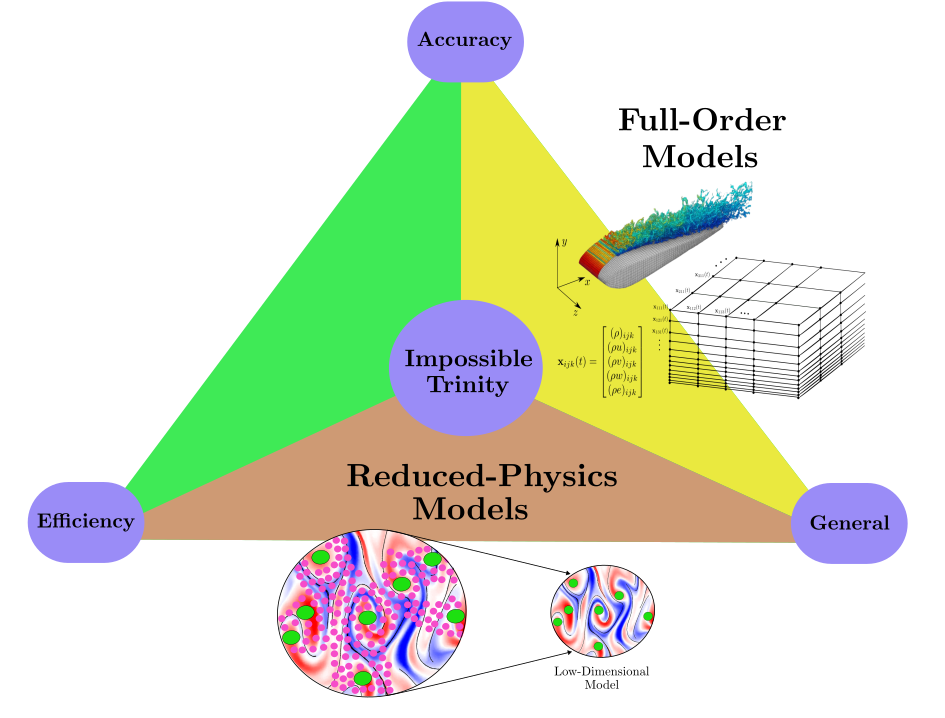
\includegraphics[width=0.8\textwidth]{../figs/introduction/itm_3.png}
                \end{figure}}
            \only<5->{
                \begin{figure}
                    \centering
                    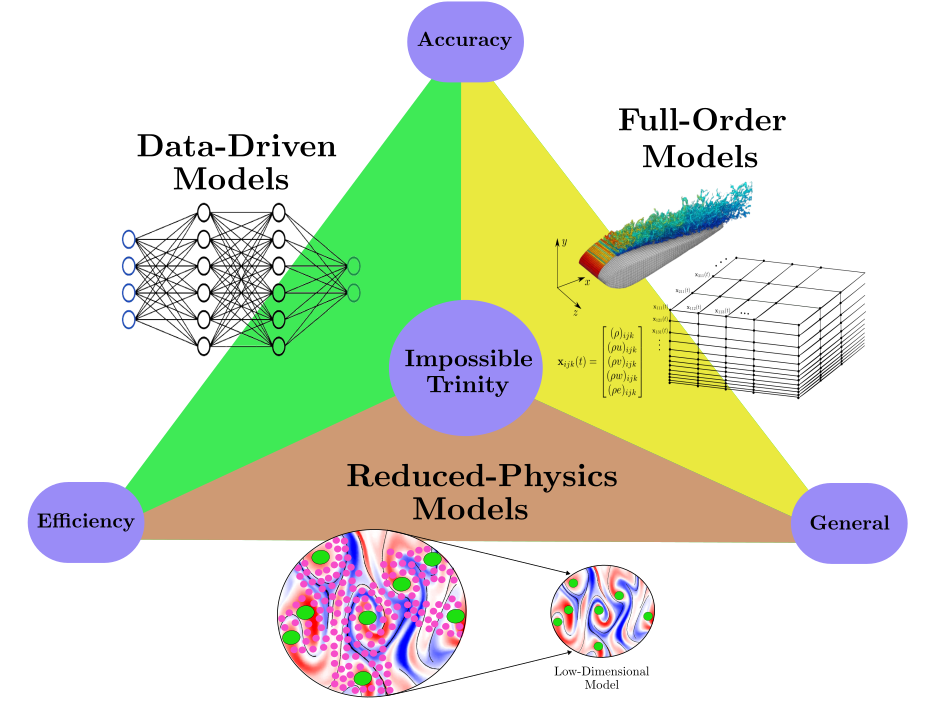
\includegraphics[width=0.8\textwidth]{../figs/introduction/itm_4.png}
                \end{figure}}
        \end{column}
        \hspace*{-0.3in}
        \begin{column}{0.46\textwidth}
            \visible<2->{
            \noindent Remains largely \textbf{unresolved} because,}
            \begin{itemize}
                \item<3-> \textbf{FEMs}: too many states,
                \item<4-> \textbf{RPMs}: overly simplified problems,
                \item<5-> \textbf{NNs}: need too much data,
            \end{itemize}
        \end{column}
    \end{columns}
    \begin{center}
        \vspace*{-0.2in}
        {\tiny ITM: Impossible Trinity of Modeling, FEM: finite-element method, RPM: reduced-physics model, NN: neural network}
    \end{center}
\end{frame}

\begin{frame}{\large ITOC: Balancing Accuracy, Efficiency, and Generalizability With Little Data}
    \footnotesize
    \begin{columns}
        \begin{column}{0.65\textwidth}
            \only<1-2>{
                \begin{figure}
                    \centering
                    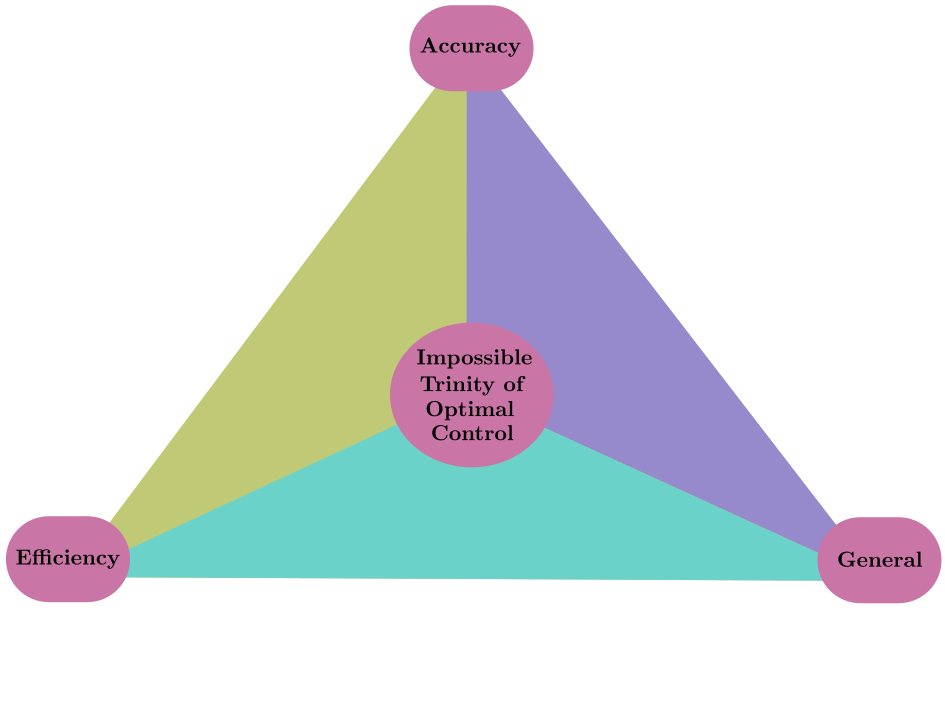
\includegraphics[width=0.8\textwidth]{../figs/introduction/itoc_1.png}
                \end{figure}}
            \only<3>{
                \begin{figure}
                    \centering
                    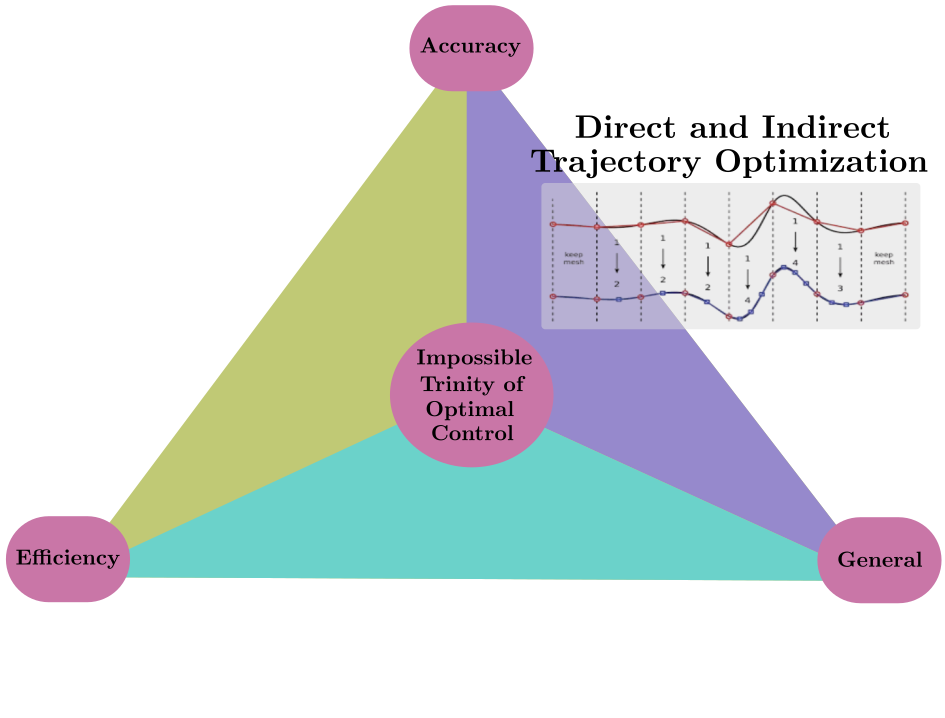
\includegraphics[width=0.8\textwidth]{../figs/introduction/itoc_2.png}
                \end{figure}}
            \only<4>{
                \begin{figure}
                    \centering
                    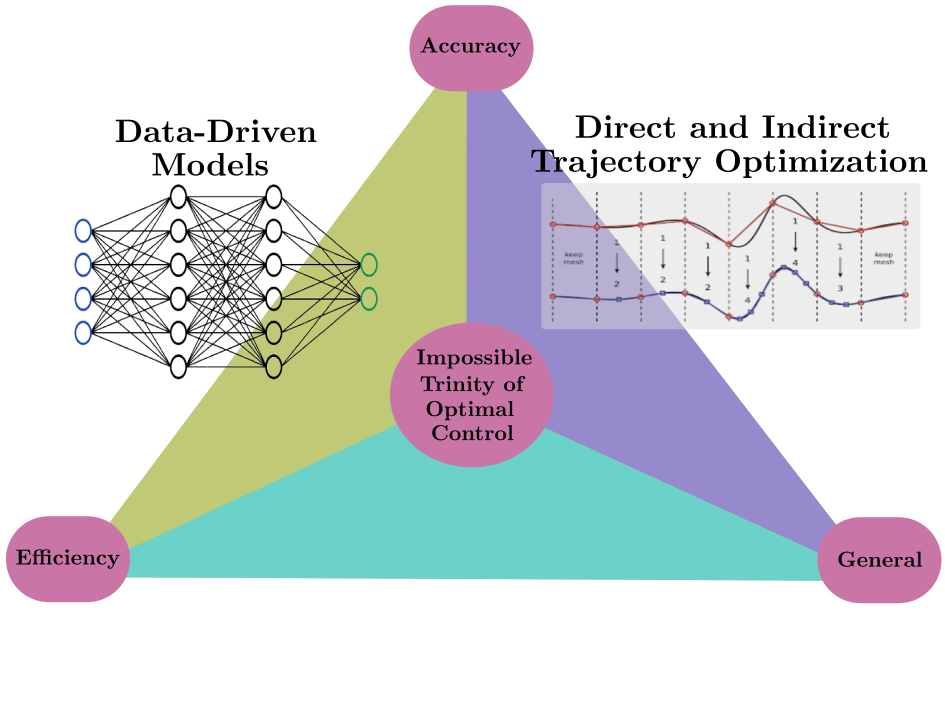
\includegraphics[width=0.8\textwidth]{../figs/introduction/itoc_3.png}
                \end{figure}}
            \only<5->{
                \begin{figure}
                    \centering
                    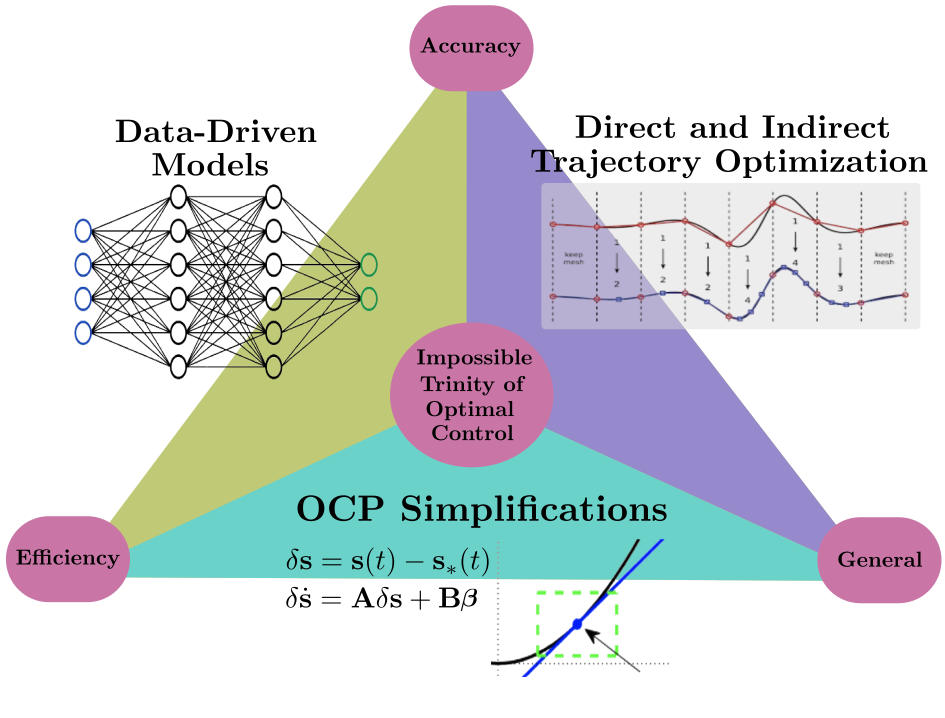
\includegraphics[width=0.8\textwidth]{../figs/introduction/itoc_4.png}
                \end{figure}}
        \end{column}
        \hspace*{-0.2in}
        \begin{column}{0.5\textwidth}
            \visible<2->{
            \noindent Remains largely \textbf{unresolved} because,}
            \begin{itemize}
                \item<3-> \textbf{TO}: need discretization and optimization,
                \item<4-> \textbf{NNs}: scarce data,
                \item<5-> \textbf{Linearizations}: not the original problem
            \end{itemize}
        \end{column}
    \end{columns}
    \visible<1->{
    \begin{center}
        {\tiny ITOC: Impossible Trinity of Optimal Control, TO: trajectory optimization, OCP: optimal control problem}
    \end{center}}
\end{frame}

\begin{frame}{\large Objectives of Research}
    \footnotesize
    \vspace*{0.1in}
    \only<1>{
        \begin{figure}
            \centering
            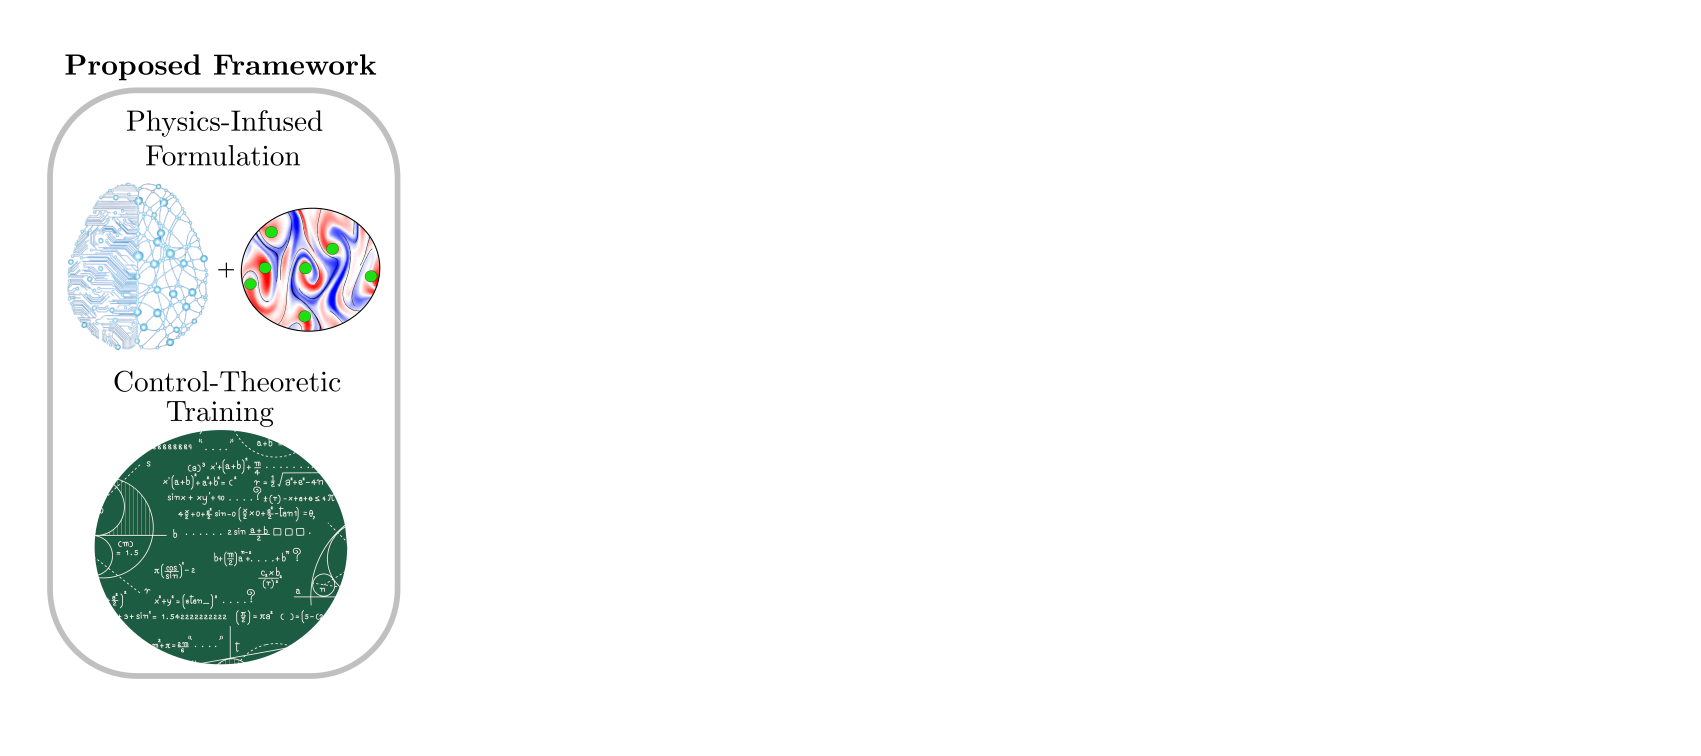
\includegraphics[width=1.0\textwidth]{../figs/introduction/objectives_1.png}
        \end{figure}}
    \only<2>{
        \begin{figure}
            \vspace*{-0.1in}
            \centering
            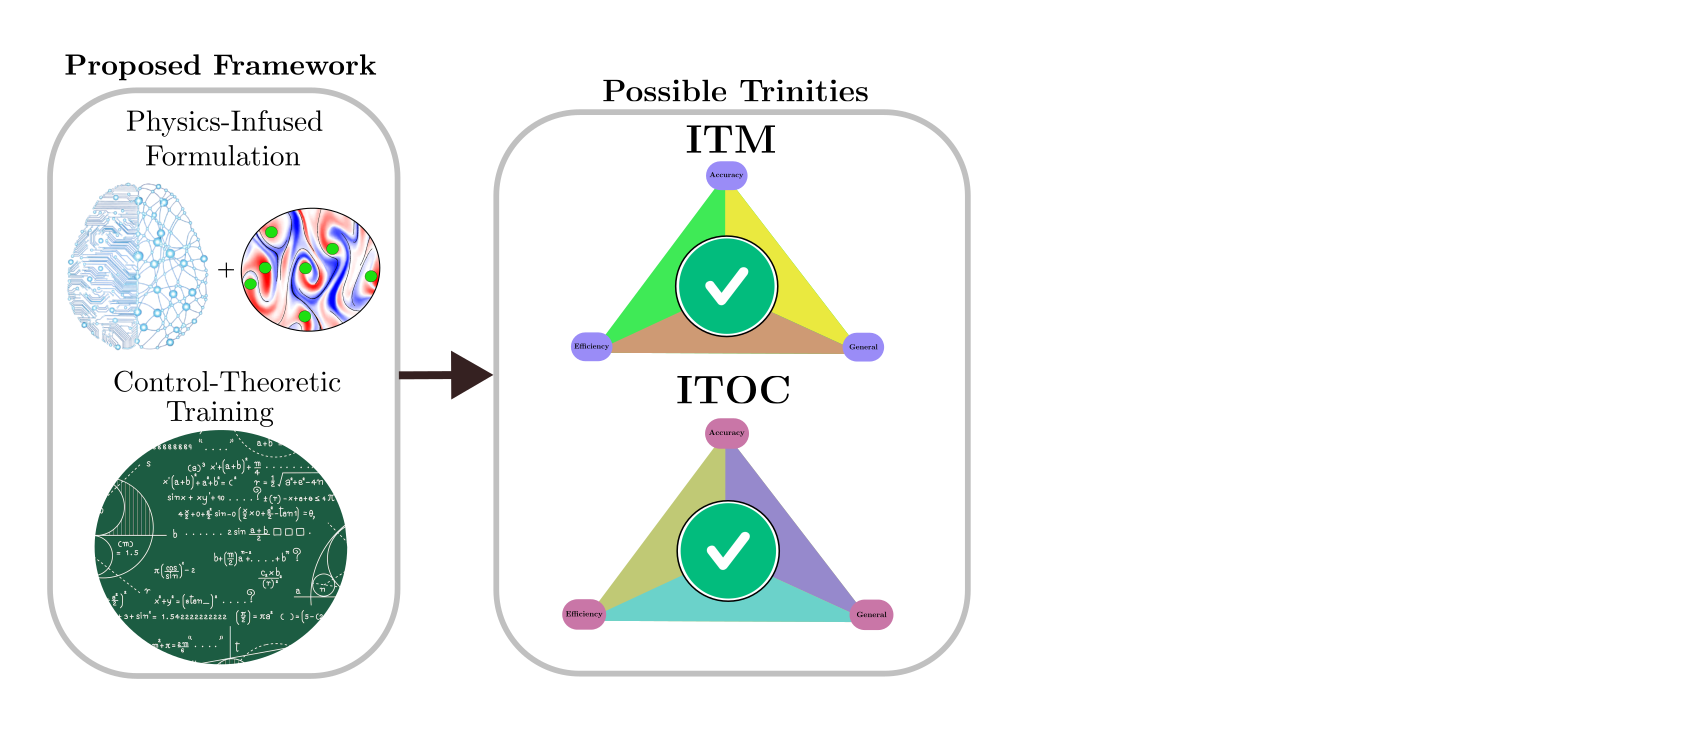
\includegraphics[width=1.0\textwidth]{../figs/introduction/objectives_2.png}
        \end{figure}}
    \only<3->{
        \begin{figure}
            \vspace*{-0.1in}
            \centering
            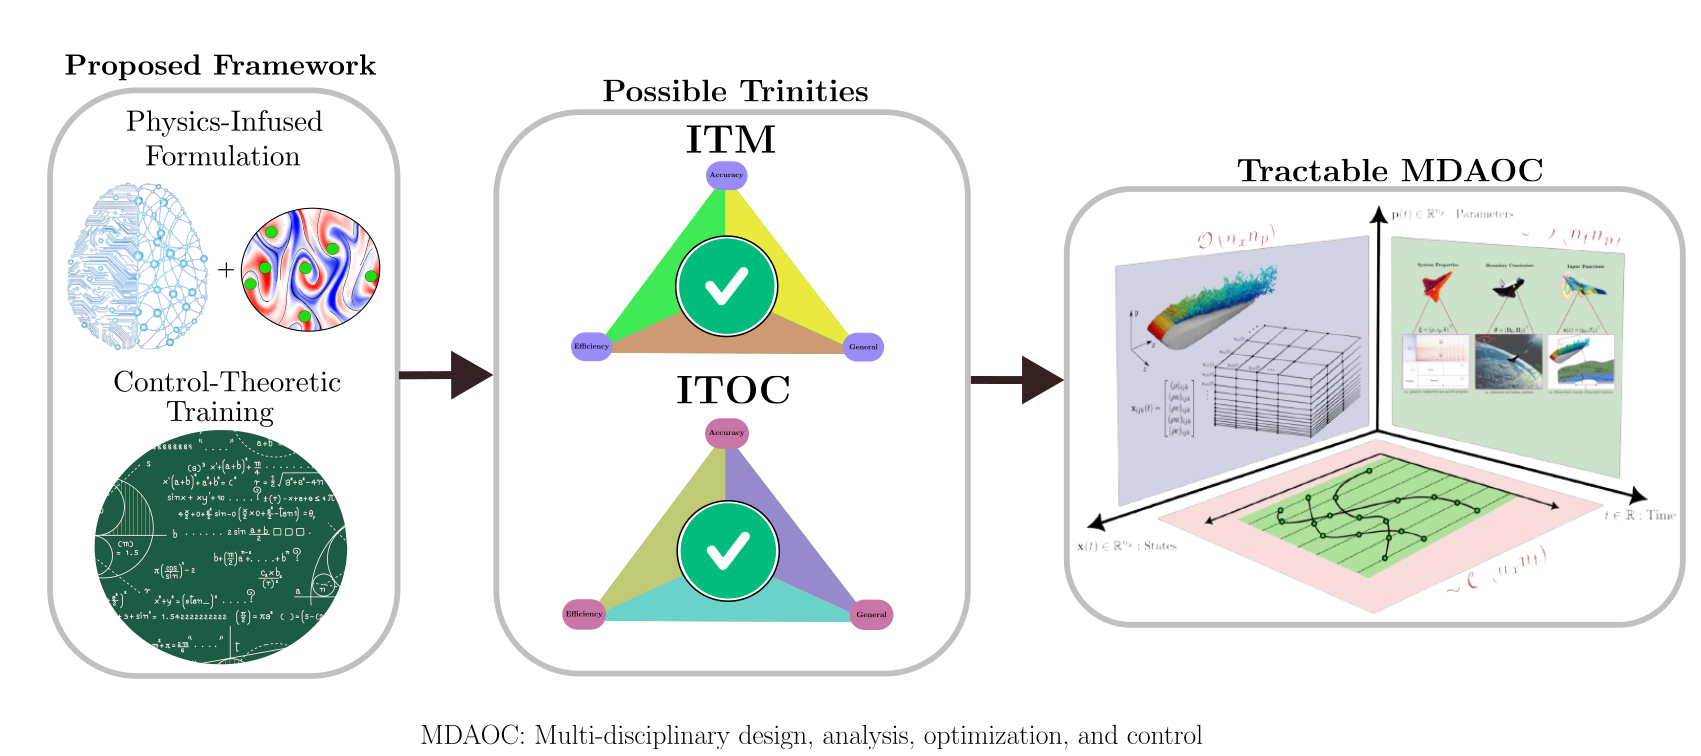
\includegraphics[width=1.0\textwidth]{../figs/introduction/objectives_3.png}
        \end{figure}}
\end{frame}
